
\chapter{Cinem\'atica}
\label{chap:1}

\section{Vectores}
\label{sec:vectores}

Las cantidades completamente especificadaw por su magnitud se llaman escalares. Ejemplos de escalares son la masa, temperatura, rapidez, etc.

Hemos visto que tanto la posici\'on, como la velocidad y la aceleraci\'on, no s\'olo tienen asociadas una magnitud, sino tambi\'en una direcci\'on. Un ejemplo de vector corresponde al asociado a la aceleraci\'on gravitacional el cual tiene una magnitud de $9.8\ \text{m}/\text{s}^2$.

\subsection{Caida libre}
La observaci\'on experimental, como por ejemplo la caida de una pluma y un bal\'\i n en un tubo de vacio, han establecido que todos los objetos cerca a la tierra se aceleran al la misma tasa constante cuando otros efectos externos est\'an excluidos.


En un sistema de coordenadas donde la direcci\'on de movimiento es perpendicular a la superficie de la tierra, podemos definir un \emph{vector unitario}, es decir, un vector de magnitud 1 y direcci\'on positiva como $\hat{\mathbf{j}}$, tal que
\begin{align}
  |\hat{\mathbf{j}}| = 1,
\end{align}
donde los simbolos $|\ |$ representan la magnitud del vector. Entonces el vector de aceleraci\'on gravitacional se puese escribir como
\begin{align}
  \mathbf{a}=-g \hat{\mathbf{j}}\,.
\end{align}

Los vectores se denotan con letra negrilla o con una flecha arriba $\vec a$. Usaremos la primera opci\'on en este texto. La magnitud del vector de aceleraci\'on gravitacional es entonces:
\begin{align}
  |\mathbf{a}|=g=9.8\ \frac{\text{m}}{\text{s}}
\end{align}

La soluci\'on a la ecuaci\'on de movimiento
\begin{align}
  \frac{d^2x(t)}{dt^2}=-g\,,
\end{align}
(con $t_0=0$) se puede escribir en forma vectorial como
\begin{align}
  \label{eq:caidalibre}
  v\,\hat{\mathbf{j}}=&(v_0-g\,t)\hat{\mathbf{j}}\nonumber\\
  y\,\hat{\mathbf{j}}=&\left(y_0+v_0\,t-\tfrac{1}{2}g\,t^2\right)\hat{\mathbf{j}}
\end{align}
de donde se puede obtener que
\begin{align}
  t=\frac{v_0-v}{g}
\end{align}
sustituyendo en ec.~\eqref{eq:caidalibre}
\begin{align}
  y-y_0=&v_0(v_0-v)/g-\tfrac{1}{2}g(v_0-v)^2/g^2\nonumber\\
       =&v_0^2/g-vv_0/g-\tfrac{1}{2}(v_0^2/g-2vv_0/g+v^2/g)\nonumber\\
       =&\tfrac{1}{2}v_0^2/g-\tfrac{1}{2}v_0^2/g\nonumber\\
       =&\tfrac{1}{2}(v_0^2-v^2)/g\,,
\end{align}
de donde,
\begin{align}
  v^2-v_0^2=-2g(y-y_0)\,,
\end{align}
esta \'ultima ecuaci\'on esta relacionada con la conservaci\'on de energ\'\i a cin\'etica m\'as energ\'\i a potencia, como se definir\'a luego.

% ver notas Kowalaski 3-11
\begin{inprogress}
  Ejemplo notas Kowalski 3-13
\end{inprogress}

\begin{itemize}
\item[\textbf{Ejemplo:}] Una piedra es lanzada hacia arriba desde lo alto de un edificio con una velocidad inicial de 20 m/s directamente hacia arriba. El edificios tiene 50 m de alto, y la piedra falla en golpear el edificio en su camino hacia abajo.
  \begin{enumerate}
  \item \textquestiondown Qu\'e tiempo le toma a la piedra alcanzar su m\'axima altura?
    \begin{align}
      v(t)=v_0-gt\,.
    \end{align}
    A la altura m\'axima $v=0$, y con $v_0=+20$ m/s
    \begin{align}
      t_{\text{max}}=&\frac{v_0}{g}\nonumber\\
      =&\frac{20}{9.8}\ s\nonumber\\
      \approx&2.04\ s
    \end{align}
  \item \textquestiondown Cual es la m\'axima altura desde la base del edificio?:\\
    Tomando el origen de coordenadas en la base del edificio:
    \begin{align}
      y_{\text{max}}=&y_0+v_o t-\frac{1}{2}g t^2\nonumber\\
      \approx&50+20\timesm2.04-\tfrac{1}{2}\timesm9.8\timesm(2.04)^2\nonumber\\
      \approx&70.4\ \text{m}\,,
    \end{align}
  \item \textquestiondown Cual es el tiempo necesario para que la piedra retorne al nivel de la torre?\\
    \begin{align}
      t_{\text{torre}}=2t_{\text{max}}\approx4.08\ \text{s}\,.
    \end{align}
  \item \textquestiondown La velocidad a ese instante?\\
    \begin{align}
      v=&v_0-gt\nonumber\\
      \approx&20-9.8\timesm4.08\\
      v_{\text{torre}}\approx&-20\ \text{m/s}\,,
    \end{align}
    La misma magnitud que la velocidad inicial pero con direcci\'on opuesta. La velocidad incial estar\'\i a representada por un vector $\mathbf{v}_0$: $\uparrow$, mientras que $\mathbf{v}_{\text{torre}}:$ $\downarrow$.
  \item \textquestiondown Cual es la velocidad y posici\'on (desde la base del edificio) despu\'es de $t=5\ \text{s}$?
    \begin{align}
      v(5)\approx 20-9.8\timesm5\approx-29.0\ \text{s}\,.
    \end{align}
    \begin{align}
      y(5)\approx50+20\timesm5-\tfrac{1}{2}\timesm9.8\timesm5^2\approx27.5\ \text{m}\,.
    \end{align}
  \item \textquestiondown Cual es la velocidad y el tiempo cuando la piedra golpea el piso?
    \begin{align}
      y_0=&50\ \text{m} & y_{\text{final}}=0\nonumber\\
      \mathbf{v}_0=&20\hat{\mathbf{j}}\ \text{m/s} & \\
    \end{align}

    \begin{align}
      v^2=&v_0^2-2g(y_{\text{final}}-y_0)\nonumber\\
      =&v_0^2-2g(0-y_0)\nonumber\\
      \approx&20^2+2\timesm9.8\timesm 50\,,
    \end{align}
de donde
\begin{align}
  \mathbf{v}_{\text{final}}=-37.1 \hat{\mathbf{j}}\ \text{m/s}\,.
\end{align}
\begin{align}
  t_{\text{final}}=&(v_0-v_{\text{final}})/g\nonumber\\
  \approx&(20+37.1)/9.8\approx5.83\,s
\end{align}
  \end{enumerate}
\end{itemize}

\subsection{Aproximaci\'on geom\'etrica a vectores}

Ejemplos de vectores: magnitud y direcci\'on
\begin{itemize}
\item Desplazamiento
\item Velocidadad
\item Aceleraci\'on
\item Fuerza
\item Momentum
\item Torque
\end{itemize}
\begin{inprogress}
  Ver ejemplo de desplazamiento en Inkscape
\end{inprogress}


Ejemplos de escalares: magnitud pero no direcci\'on
\begin{itemize}
\item Longitud
\item Tiempo
\item Masa
\item \'Area
\item Volume
\item Densidad
\item Energ\'\i a
\item Temperatura
\end{itemize}

\begin{align}
  \mathbf{A}=&\mathbf{B} & \text{si}\quad |\mathbf{A}|=
  |\mathbf{B}|\,.
\end{align}
Adem\'as
\begin{align}
  A\equiv|\mathbf{A}|\,.
\end{align}

\textbf{Suma de vectores}
Cabeza y cola
\begin{inprogress}
  inkscape: ley conmutativa
\end{inprogress}
Suma s\'olo tiene sentido para el mismo para el mismo tipo de vectores
\subsection{Aproximaci\'on algrebr\'aica  a vectores}

\begin{frame}[fragile,allowframebreaks]
Un vector en el plano $x-y$, con vectores unitarios $\hat{\mathbf{i}}$ en la direcci\'on $x$, $\hat{\mathbf{j}}$ en la direcci\'on $j$, y  formando un \'angulo $\theta$ con el eje $x$ se puede visualizar como la suma de dos vectores:
\begin{align}
  \mathbf{A}=&\mathbf{A}_x+\mathbf{A}_y\nonumber\\
            =&A_x\hat{\mathbf{i}}+A_y\hat{\mathbf{j}}\nonumber\\
            =&(A_x,A_y)\nonumber\\
            =&(A_1,A_2).
\end{align}
En t\'erminos de componentes
\begin{align}
  \mathbf{A}_i=A_i\,.
\end{align}
La magnitud al cuadrado del vector se obtiene del teorema de Pitagoras
\begin{align}
  \label{eq:pitagoras}
  \mathbf{A}\cdot\mathbf{A}\equiv|\mathbf{A}|^2=A^2=&A_x^2+A_y^2\nonumber\\
  =&\sum_{i=1}A_i^2\,.
\end{align}
Definiendo el delta de Kronecker como
\begin{align}
  \delta_{ij}=
  \begin{cases}
    1&\text{si $i=j$}\\
    0&\text{si $i\neq j$}\\
  \end{cases}
\end{align}
podemos escribir la magnitud al cuadrado del vector $\mathbf{A}$ de una forma que se puede generalizar facilmente a $n$-dimensiones:
\begin{align}
   A^2=\mathbf{A}\cdot\mathbf{A} =&\sum_{i,j=1}A_i A_j\delta_{ij}\nonumber\\
   =&\sum_{i=1}^2\left(A_iA_1\delta_{i1}+A_iA_2\delta_{i2}+A_iA_1\delta_{i3}\right)\nonumber\\
   % falta un paso
   =&A_1A_1\delta_{11}+A_2A_2\delta_{22}+A_3A_3\delta_{33}\nonumber\\
   =&A_1^2+A_2^2+A_3^2\nonumber\\
   =&\sum_{i=1}A_i^2\,.
\end{align}
Teniendo en cuenta el \'angulo $\theta$ en la ec.\eqref{eq:pitagoras} tenemos que
\begin{align}
  A_x=&|\mathbf{A}|\cos\theta=A\cos\theta\nonumber\\
  A_y=&|\mathbf{A}|\sin\theta=B\sin\theta\,,
\end{align}
De modo que
\begin{align}
  \tan\theta=\frac{A_y}{A_x}\,,
\end{align}
y
\begin{align}
  \theta=\tan^{-1}\frac{A_y}{A_x}
\end{align}


Para sumar dos vectores algebra\'\i camente, se desplazan los origines de los dos vectores a un origin de coordenadas que coincida con el plano formado por los dos vectores. Entonces es facil ver que
\begin{align}
  \mathbf{C}=\mathbf{A}+\mathbf{B}=&(A_x+B_x)\hat{\mathbf{i}}+(A_y+B_y)\hat{\mathbf{j}}\nonumber\\
  =&(A_x+B_x,A_y+B_y)\nonumber\\
  =&(A_1+B_1,A_1+B_1).
\end{align}
En t\'erminos de componentes:
\begin{align}
  \left(\mathbf{A}+\mathbf{B}\right)_i=A_i+B_i\,.
\end{align}
\end{frame}

\begin{frame}[fragile,allowframebreaks]
Para visualizar el producto escalar definimos $\beta$ como el \'angulo entre
los vectores $\mathbf{A}$ y $\mathbf{B}$. Escojemos el sistema de
coordenadas en el plano formado por los dos vectores tales que $\alpha+\beta$
sea el \'angulo de $\mathbf{A}$ con $x$ y $\alpha$ el \'angulo de $\mathbf{B}$,
entonces, de la definici\'on
\begin{align}
  \mathbf{A}\cdot\mathbf{B}\equiv&A_xB_x+A_yB_y\nonumber\\
  =&\sum_{i,j=1}^2A_iB_j\delta_{ij}\nonumber\\
  =&\sum_{i}^2A_iB_i\,,
\end{align}
tenemos:
\begin{align}
    \mathbf{A}\cdot\mathbf{B}=&A_xB_x+A_yB_y\nonumber\\
    =&A\cos(\alpha+\beta)B\cos\alpha+A\sin(\alpha+\beta)B\sin\alpha\nonumber\\
    % Faltan detallaes
    =&AB\cos\beta\nonumber\\
    =&|\mathbf{A}||\mathbf{B}|\cos\beta\,,
\end{align}
como era de esperarse. De este modo, el \'angulo entre dos vectores,
$\beta$, se puede obtener como
\begin{align}
  \cos\beta=\frac{\mathbf{A}\cdot\mathbf{B}}{|\mathbf{A}||\mathbf{B}|}\,.
\end{align}
\end{frame}

\begin{frame}[fragile,allowframebreaks]
El producto vectorial $\mathbf{C}=\mathbf{A}\timesm\mathbf{B}$, se define algebra\'\i camente como:
\begin{align}
  C_k=\left(\mathbf{A}\timesm\mathbf{B}\right)_k=&\sum_{ij}\epsilon_{ijk}A_iB_j\,,
\end{align}
donde el s\'\i mbolo de Levi-Civita se define con respecto a las
permutaciones con referencia al orden 123 como
\begin{align}
  \epsilon_{ijk}\equiv& \begin{cases}
    0&\text{si hay \'\i ndices iguales}\\
    1&\text{permutaci\'on par}\\
    -1&\text{permutaci\'on impar}\\
  \end{cases}.
\end{align}
Entonces
\begin{align}
  C_x=C_1=\left(\mathbf{A}\timesm\mathbf{B}\right)_1=&
\sum_{i=1}^3\left(\cancel{\epsilon_{i11}}A_iB_1+\epsilon_{i21}A_iB_2+\epsilon_{i31}A_iB_3\right)\nonumber\\
=&\cancel{\epsilon_{121}}A_1B_2+\cancel{\epsilon_{221}}A_2B_2
+\epsilon_{321}A_3B_2+\cancel{\epsilon_{131}}A_1B_3\nonumber\\
&+\epsilon_{231}A_2B_3+\cancel{\epsilon_{331}}A_3B_3\,.
\end{align}
Teniendo en cuenta que $321\to231\to213\to123$ (3 permutaciones) y
$231\to213\to123$ (2 permutaciones), entonces
\begin{align}
  \epsilon_{321}=-1\,\qquad \epsilon_{231}=+1\,,
\end{align}
entonces
\begin{align}
  C_x=C_1=&A_2B_3-A_3B_2\,.
\end{align}
Similarmente para $C_y$ y $C_z$, tenemos
%faltan detalles
\begin{align}
  \label{eq:crossprod}
  \mathbf{C}=&\left(A_yB_z-A_zB_y\right)\hat{\mathbf{i}}
-\left(A_xB_z-A_zB_x\right)\hat{\mathbf{j}}
+\left(A_xB_y-A_yB_x\right)\hat{\mathbf{k}}\nonumber\\
 =&\left(A_2B_3-A_3B_2,A_3B_1-A_1B_3,A_1B_2-A_2B_1\right)
\,.
\end{align}
Definimos
\begin{align}
  \label{eq:det}
  \mathbf{C}=\begin{vmatrix}
    \hat{\mathbf{i}} & \hat{\mathbf{j}} & \hat{\mathbf{k}}\\
    A_x & A_y & A_z\\
    B_x & B_y & B_z
  \end{vmatrix}\equiv\left(A_yB_z-A_zB_y\right)\hat{\mathbf{i}}
-\left(A_xB_z-A_zB_x\right)\hat{\mathbf{j}}
+\left(A_xB_y-A_yB_x\right)\hat{\mathbf{k}}\,.
\end{align}
El resultado (\ref{eq:crossprod}) se puede obtener tambi\'en con la
regla para calcular el determinante definido en la ec.~(\ref{eq:det}),
como se muestra en la figura~\ref{fig:cross}.
\begin{figure}
  \centering
  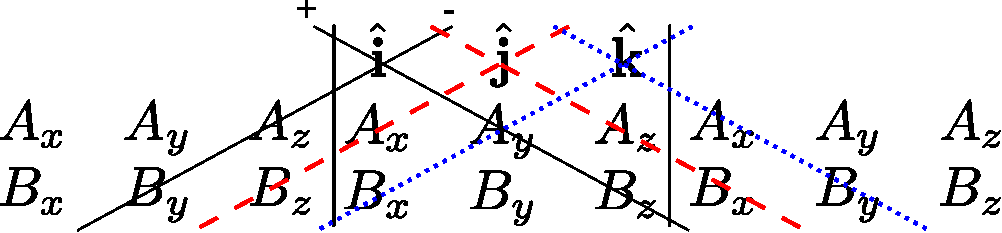
\includegraphics[scale=0.7]{cross}
  \caption{Regla para el determinante: Para cada par de l\'\i neas, el cruze de las l\'\i neas definen
    el vector unitario, que va acompa\~nado por el producto de las
    cantidades bajo la l\'\i nea de izquierda  a derecha menos el producto
    de la cantidades de derecha a izquierda. El signo menos aparece
    naturalmente para el producto asociado a $\hat{\mathbf{j}}$.  }
  \label{fig:cross}
\end{figure}

Para mostrar como el producto vectorial se reduce la definici\'on
geom\'etrica en t\'erminos de las magnitudes y el \'angulo entre los dos
vectores, considere el plano definido por los vectores $\mathbf{A}$ y
$\mathbf{B}$ que forman un \'angulo $\alpha$ entre ellos. Escojamos el eje
$x$ a lo largo del vector $\mathbf{A}$. Entonces:
\begin{align}
  A_y=A_z=B_z=0\qquad A=A_x\qquad\text{y}\ B_y=B\sin\alpha\,. 
\end{align}
Por consiguiente
\begin{align}
  \mathbf{C}=\mathbf{A}\timesm\mathbf{B}=&A_xB_y\hat{\mathbf{k}}\nonumber\\
  =&A B\sin\alpha\,\hat{\mathbf{k}}\,,
\end{align}
y entonces
\begin{align}
  |\mathbf{C}|=|\mathbf{A}||\mathbf{B}|\sin\alpha\,.
\end{align}
\end{frame}



%\left(\right)
%ver inkscape vectores primera capa






%%% Local Variables: 
%%% mode: latex
%%% TeX-master: "mecanica"
%%% End: 
